\subsection{A Baseline System}

For this paper, I solve the system in \autocites{othmer2009intersection}{jeong2017numerical}. By replacing the reaction function, the method can be extended to any sufficiently smooth reaction-diffusion system. This includes Turing's initial version \parencites{turing1990chemical}{de2020leopard} and other activator-inhibitor equations \parencites{landge2020pattern}{meinhardt2000pattern} which it has been tested against. The system I solve is given by
\begin{align*}
    \frac{\partial u}{\partial t} = \gamma_u \nabla^2 u + k_1 \left(v - \frac{uv}{1 + v^2}\right) \\
    \frac{\partial v}{\partial t} = \gamma_v \nabla^2 v + k_2 - v - \frac{4 u v}{1 + v^2}.
\end{align*}

Like \autocite{jeong2017numerical}, I fix $D_u = 1$ and $k_2 = 11$ in all simulations. I vary $D_v$ and $k_1$ across simulations to create different Turning patterns, but we always have $D_v< D_u$. The time step is set to $\Delta t = 0.01$, and all systems are iterated until $t = 1,000$, at which point they all have reached a steady state. I triangulate so that there are 250 points per square unit of the domain I solve the PDE on. The plotted solutions will be of $u$, although $v$ makes a similar pattern.


\subsection{Solutions}

\begin{figure}[t!]
    \centering
    \caption{Solutions to the reaction-diffusion system}

    \begin{subfigure}{\textwidth}
        \centering
        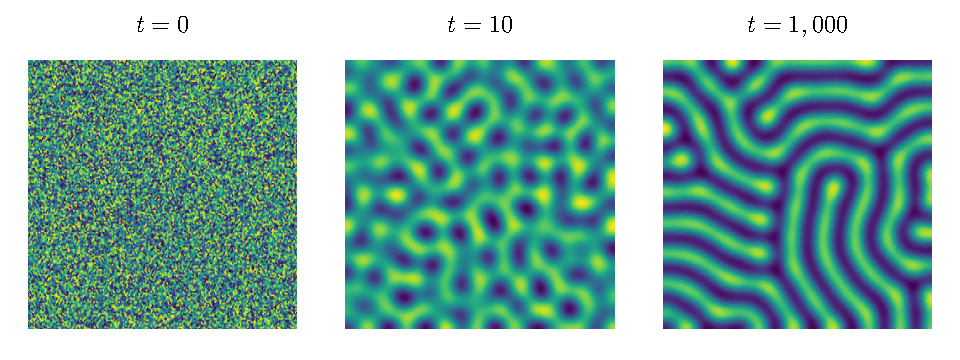
\includegraphics{figures/square_ts.pdf}
        \caption{$10 \times 10$ square domain}
    \end{subfigure}

    \begin{subfigure}{\textwidth}
        \centering
        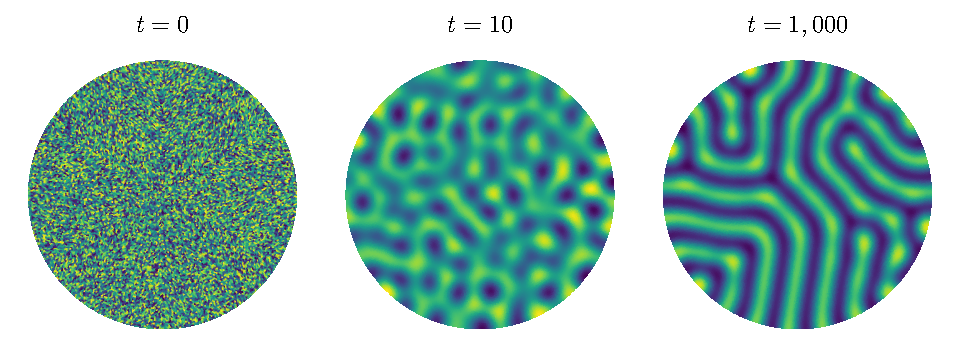
\includegraphics{figures/circle_ts.pdf}
        \caption{Radius 5 circular domain}
    \end{subfigure}

    \label{fig:sol-ts}
\end{figure}

Figure \ref{fig:sol-ts} plots the solution to the reaction-diffusion system at different time steps on a square and circular domain. The left panel plots the initial condition, the middle panel plots an intermediate step during the reaction, and the right panel plots the system at steady state. I set the initial condition to random noise. At $t = 10$, the reaction starts to progress, and we see patterns and `hotspots' emerge. The patterns that exist, however, lack clear definition. In the steady state, we see well-defined lines that form clear Turing patterns.

At each time step, the system makes similar shapes on the circular and square domains. The intermediate step patterns both have similarly sized hotspots, and the Turing patterns that develop have a similar structure being made of curved-lines with similar width. I explore this further in Section \ref{sec:doms} with more complicated domains and arrive at the same result.


\subsection{Parameters}

The chosen parameterization has significant effects on the shape of the Turing patterns that develop. Specifically, alternate choices for the diffusion coefficient for $v$ and the feed concentration $k_1$ can change significant features of the patterns.

\begin{figure}[t!]
    \centering
    \caption{$10 \times 10$ square steady states for different $\gamma_v$ and $k_1$}
    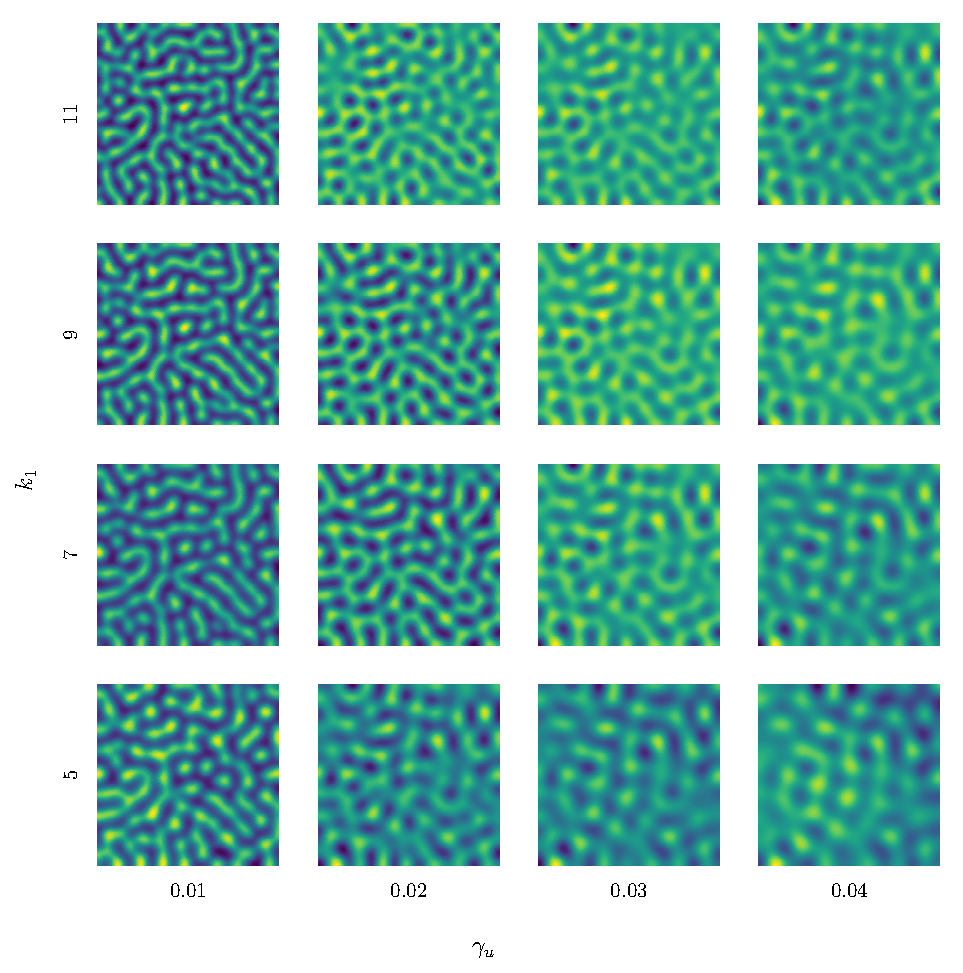
\includegraphics{figures/square_params.pdf}
    \label{fig:sq-pars}
\end{figure}

Figure \ref{fig:sq-pars} shows how parameter choice affects the Turing patterns in $\gamma_v - k_1$ space on a square domain. With higher diffusion, the patterns are less defined having more fuzziness along the boundary and are wider. With low $\gamma_v$, spots emerge since the diffusion is not strong enough to merge the disjoint elements together. Increasing $k_1$ merges the spots together again forming stripes, but does not have the same effect on the width and definition of the patterns. With high $\gamma_v$ and $k_1$ the patterns become dominated by high-concentrations of $u$ (yellow) instead of low concentrations (purple).

\begin{figure}[t!]
    \centering
    \caption{Radius 5 circle steady states for different $\gamma_v$ and $k_1$}
    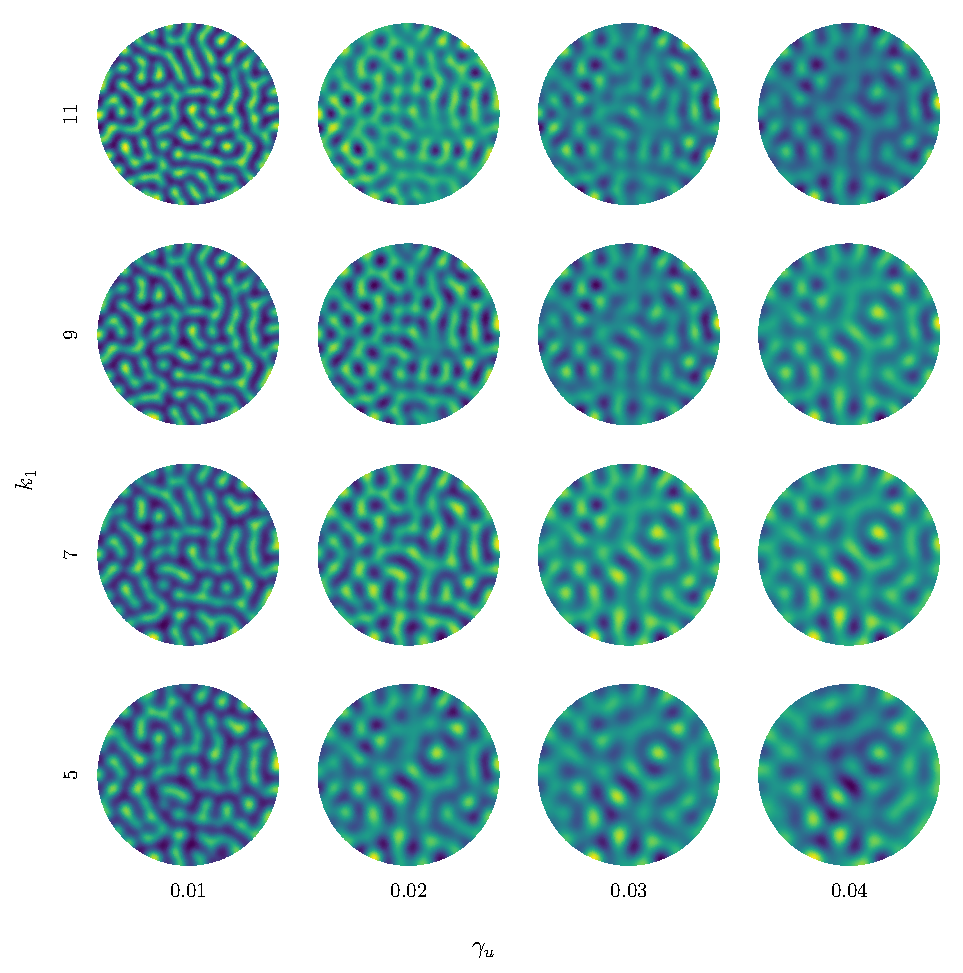
\includegraphics{figures/circle_params.pdf}
    \label{fig:cir-pars}
\end{figure}

The parameterization has the same effect on alternate domains. Figure \ref{fig:cir-pars} shows the same parameterizations on a circular domain. Higher $\gamma_v$ similarly increases the width and decreases the definition of the Turing patterns, and higher $k_1$ merges the patterns together to form lines.


\subsection{Error Analysis} \label{subsec:err}

By discretizing the grid, I am introducing potential numerical error into the solution. I analyze this by comparing solutions on less granular triangulations to the solution on a very fine triangulation. Denoting $\hat{u}^{N}$ the finite element approximation for $u$ on a grid with an average of $N$ vertices along a 1 unit path across edges in the triangulation, I calculate
\[
    \epsilon_N = \int_\Omega \left| \hat{u}^N (\overline{t}, x, y) - \hat{u}^{\overline{N}} (\overline{t}, x, y) \right| dA
\]
for some large $\overline{t}$ so that the system has reached the steady state and large $\overline{N}$ to get as accurate an approximation as possible of the exact solution. I use $\overline{N} = 50$, which means each square unit in the domain has approximately 2,500 vertices in it. I evaluate $\hat{u}^N$ with $k_1 = 9$ and $\gamma_v = 0.02$ on an evenly spaced $100 \times 100$ grid then use a Riemann sum to calculate the integral. For the initial condition, I use OpenSimplex noise \autocite{thorimbert2016polynomial}. This ensures all $N$ have the same $u$ at $t = 0$.

\begin{figure}[t!]
    \centering
    \caption{Numerical error in the solutions on a $10 \times 10$ square domain}

    \begin{subfigure}{\textwidth}
        \centering
        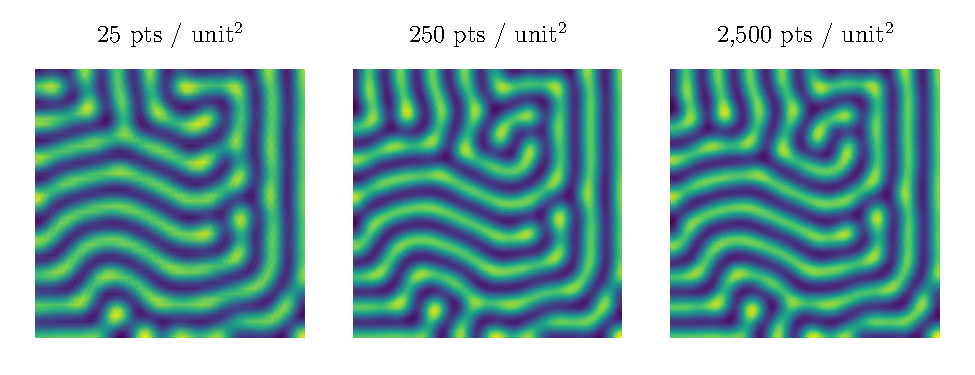
\includegraphics{figures/error.pdf}
        \caption{Calculated steady state with different $N$}
        \label{subfig:res-by-N}
    \end{subfigure}

    \begin{subfigure}{\textwidth}
        \centering
        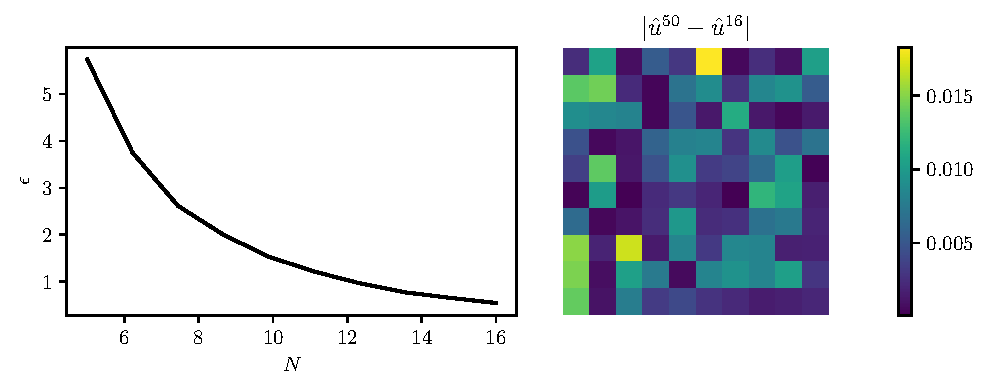
\includegraphics{figures/err_ovr_N.pdf}
        \caption{(Left) Error by $N$; (Right) Error over $\Omega$ for $N = 16$}
        \label{subfig:err-over-N}
    \end{subfigure}

    \label{fig:err}
\end{figure}

Figure \ref{fig:err} gives the results of this analysis. Panel \ref{subfig:res-by-N} shows the resulting steady states using different $N$. Qualitatively, the Turing patterns that develop look very similar across $N$. With low $N$, the lines do form different connections, especially in the top right corner where the lines form together differently when $N = 16$ and $N = 50$ versus when $N = 5$. The patterns in the $N = 16$ and $N = 50$ case are visually identical.

Panel \ref{subfig:err-over-N} shows the total error for different values of $N$ and the comparison between the $N = 16$ and $N = 50$ case. In general, a larger value of $N$ reduces error, although there is diminishing returns since the magnitude of the error decrease is lower at higher $N$. For the $N = 16$ case, total error is low across the whole domain. The error follows wave-like patterns through the domain. Comparing the locations of the error with the patterns in Panel \ref{subfig:res-by-N}, the points with the highest error are located on the boundaries of the Turing patterns. This is consistent with the fact that the FEM approximation is worse in areas where the function is less smooth.
